\documentclass{ctexart}
\usepackage{graphicx}
\graphicspath{{./img}}
\usepackage{amsmath}

\author{梁伟德\\ 21215193}
\title{探究作业1:\\\textbf{高斯波包耗散}}

\newcommand{\bra}[1]{\langle #1 |}
\newcommand{\ket}[1]{|#1\rangle}
\newcommand{\bk}[2]{\langle #1 | #2 \rangle}
\newcommand{\h}[1]{\hat{#1}}
\newcommand{\hd}[1]{\hat{#1}^{\dagger}}
\begin{document}

\maketitle
问题如图\ref{fig:homework}。
\begin{figure}[h]
    \centering
    \caption{作业}\label{fig:homework}
    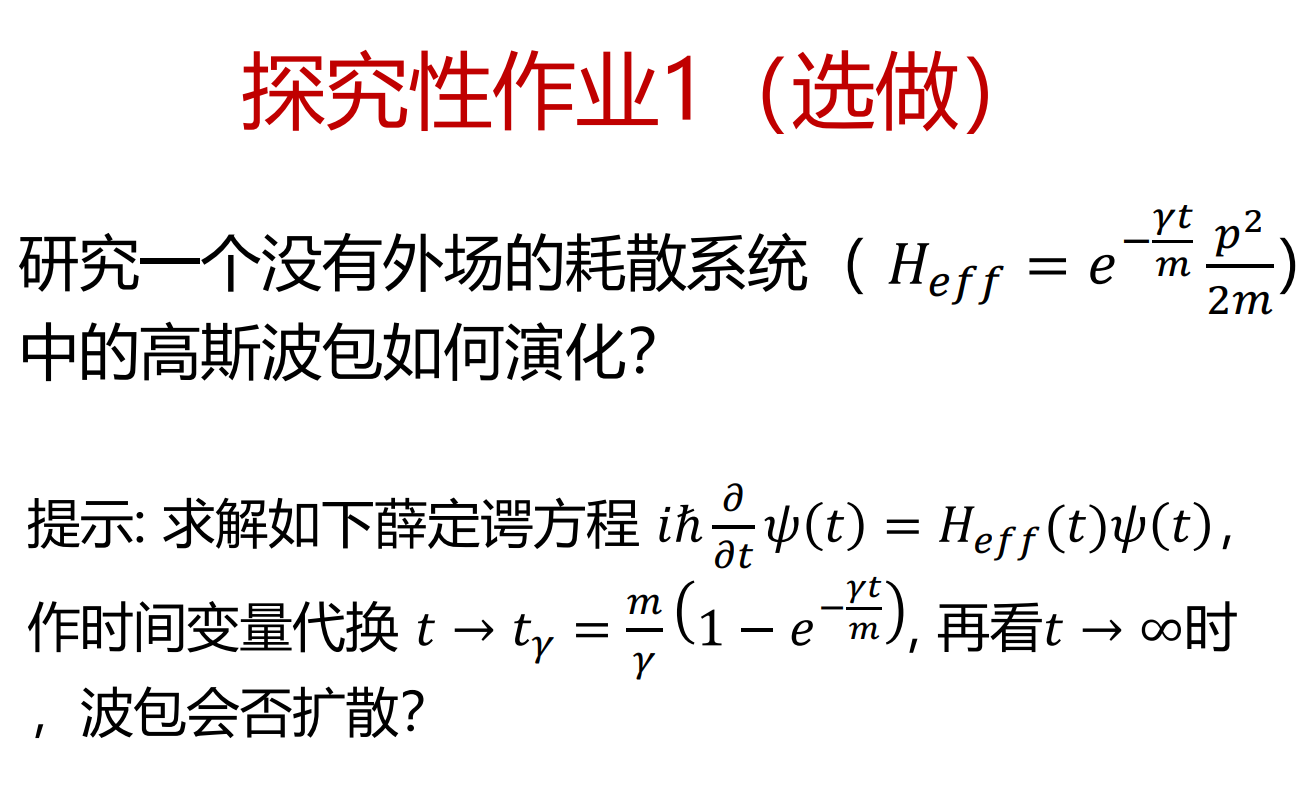
\includegraphics[width = 0.8\textwidth]{Snipaste_2021-10-15_18-38-55.png}
\end{figure}
\par

对于系统的薛定谔方程有:
\begin{equation}
    i\hbar = \frac{\partial}{\partial} \ket{\Psi} = \hat{H}_{eff} \ket{\psi}
\end{equation}
对于这种不同时间哈密顿量相互对易的方程,演化算符有简单形式的解:
\begin{align}
    \h{U}(t,0) &= exp\{-\frac{i}{\hbar}\int_0^{t} dt' e^{\textstyle \frac{\gamma t'}{m}} \frac{p^2}{2m}\} \notag\\
    &= e^{\textstyle -\frac{i}{\hbar} \frac{\h{p}^2}{2m} t_{\gamma}}  \\
    where \quad & t_{\gamma} = \frac{m}{\gamma}(1-e^{\textstyle -\frac{\gamma t}{m}}) \notag
\end{align}
从这里可以看出,$t \rightarrow \infty, t_{\gamma} \rightarrow \frac{m}{\gamma}$。
所以在这个近似哈密顿量的描述下,波包永远不会耗散消失,最终只会趋于一个较宽的分布。\par

已知高斯波包在动量表象下的形式为:
\begin{equation}
    \psi(p) = \sqrt{\frac{d}{\hbar\sqrt{\pi}}}\ e^{\textstyle -\frac{p^2d^2}{2\hbar^2}}
\end{equation}
\begin{align}
    \ket{\psi(t)} &= e^{\textstyle -\frac{i}{\hbar} \frac{\h{p}^2}{2m} t_{\gamma}} \ket{\psi}  \notag\\
    &= e^{\textstyle -\frac{i}{\hbar} \frac{\h{p}^2}{2m} t_{\gamma}} \sqrt{\frac{d}{\hbar\sqrt{\pi}}}e^{\textstyle -\frac{p^2d^2}{2\hbar^2}} \notag\\
    &= \sqrt{\frac{d}{\hbar\sqrt{\pi}}}\ e^{\textstyle -p^2(\frac{it_{\gamma}}{2m\hbar} + \frac{d^2}{2\hbar^2})}
\end{align}
再将动量波函数做逆傅立叶变换回到坐标波函数:
\begin{align}
    \psi(x) &= \frac{1}{\sqrt{2\pi\hbar}}\int_{-\infty}^{+\infty}dp\ e^{\textstyle ipx/\hbar}\ \psi(p) \notag \\
    &= \sqrt{\frac{d}{2\sqrt{\pi}}} \sqrt{\frac{2m}{it_{\gamma}\hbar + md^2}}\ e^{\textstyle -\frac{x^2}{4c\hbar^2}} \\
    where \qquad & c = \frac{it_{\gamma}}{2m\hbar} + \frac{d^2}{2\hbar^2}
\end{align}
\end{document}